\subsection{Framework}
% Resumen de https://tools.ietf.org/id/draft-opsawg-ntf-00.html

\subsubsection{Mecanismos de adquisición de datos}

En general, los datos de red se pueden obtener mediante subscripción (push) o consulta(poll). A su vez existen dos modelos de subscripción, Publish-Subscription y Subscription-Publish. En el perimero, una serie de datos predefinidos están publicados y varios subscriptores pueden solicitar esos datos. En el otro modo, un subscriptor comunica que datos quiere obtener y los dispositivos de red son los encargados de entregar esos datos cuando sean disponibles.

En cambio, un agente que realiza pooling espera una respuesta inmediata por parte de los dispositivos de red. 

Existen 4 tipos de datos que puede proporcional un dispositivo de red:
\begin{itemize}
    \item \textbf{Datos Simples}: datos que están siempre disponibles desde algún almacén de datos o sondas estáticas del dispositivo de red. Este tipo de datos puede ser especificado mediante un modelo YANG
    \item \textbf{Datos personalizados}: Estos datos necesitan ser sintetizados o procesados a partir de datos en bruto procedentes de uno o varios dispositivos de red.
    \item \textbf{Datos basados en eventos}: Los datos se generan condicionalmente en base a algún evento.
    \item \textbf{Datos de flujo}: Estos datos están siendo generados continuamente o de forma periódicamente.Los datos de flujo muestran el estado de un dispositivo real y requieren mucho ancho de banda y poder de procesamiento.
\end{itemize}

Como puede verse en la Figura \ref{fig:tipos_de_datos_framework} estos tipos de datos no nos excluyentes.

\begin{figure}
    \centering
    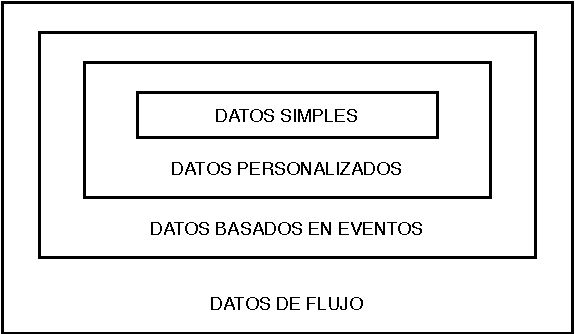
\includegraphics[scale=.75]{graphics/tipos_de_datos_framework}
    \caption{Relaciones entre los tipos de datos}
    \label{fig:tipos_de_datos_framework}
\end{figure}

En general las subscripciones trabajan con datos de flujo o datos basados en eventos mientras que el polling se usa más para datos simples o datos personalizados.


\subsubsection{Data Objects}
La telemetría se puede dividir también en cuatro módulos, en función del origen de los datos:

\begin{itemize}
    \item \textbf{Control Plane Telemetry}
    \item \textbf{Forwarding Plane Telemetry}
    \item \textbf{Management Plane Telemetry}
    \item \textbf{External Data and Event Telemery}
\end{itemize}


Las principales diferencias entre los 4 modulos los podemos ver en la Tabla \ref{tab:diferencias_modulos_data_objects}:
\begin{table}
    \centering
    \begin{tabular}{|p{2cm}|p{3cm}|p{3cm}|p{3cm}|p{3cm}|}
        \hline
        \textbf{Module} & \textbf{Control Plane} &\textbf{Management Plane} & \textbf{Forwarding Plane} & \textbf{External Data} \\\hline
        
        \textbf{Object} & control protocol \& signaling, RIB, ACL & config, operation state, MIB & flow \& packet QoS, trafic stat., buffer \& queue stat & terminal, social \& environmental\\\hline
        
        \textbf{Export Location }& main control CPU, linecard CPU or fwding chip & main control CPU & fwding chip or linecard CPU; main control CPU unlikely & various \\\hline
        
        \textbf{Model} & YANG, custom & MIB, syslog, YANG, custom & template, YANG custom & YANG\\\hline
        
        \textbf{Encoding} & GPB, JSON, XML, plain & GPB, JSON, XML & plain &  GPB, JSON, XML, plain\\\hline
        
        \textbf{Protocol} & gRPC, NETCONF, IPFIX, mirror & gRPC, NETCONF& IPFIX, mirror & gRPC\\\hline
        
        \textbf{Transport} & HTTP, TCP, UDP & HTTP, TCP & UDP & TCP, UDP \\\hline
        
        
        \end{tabular}

    \caption{Diferencias entre módulos del framework de telemetría de red}
    \label{tab:diferencias_modulos_data_objects}
\end{table}






\subsubsection{Evolución de la telemetría de red}
De la misma forma que las redes tienden a evolucionar hacia una forma de operar mucho más autónoma, la telemetría de red también se puede clasificar en varios niveles en función del nivel de autonomía:
\begin{enumerate}[label=Nivel \arabic*, leftmargin=4\parindent]
    \setcounter{enumi}{0}
    \item \textbf{Telemetría estática}: Los datos de telemetría se fijan en la fase de diseño.
    \item \textbf{Telemetría Dinámica}: Los datos de telemetría se pueden programar y configurar de forma dinámica en tiempo de ejecución.
    \item \textbf{Telemetría Interactiva}: Un operador de red puede alterar en tiempo real la telemetría. A este nivel algunas tareas se pueden automatizar aunque siempre se necesita un operador humano para tomar decisiones.
    \item \textbf{Circuito-Cerrado}: No hay operadores humanos. La red es inteligente y su sistema de control solicita datos de telemetría automáticamente, analiza los datos y modifica el funcionamiento de la red.
\end{enumerate}

La mayoría de las tecnologías existentes operan en el nivel 0 o 1 pero con la ayuda de un framework de telemetría bien definido se pueden crear las tecnologías para dar soporte al nivel 2 y dar los primeros pasos hacía el nivel 3.



\subsection{Network Configuration Notifications\label{sec:NETCONFNot}}

https://tools.ietf.org/html/rfc5277

\subsection{YANG Push Notifications\label{sec:YANGNot}}

https://datatracker.ietf.org/doc/rfc8641/
https://tools.ietf.org/id/draft-ietf-netconf-notification-capabilities-05.html